%%%%%%%%%%%%%%%%%%%%%%%%%%%%%%%%%%%%%%%%%%%%%%%%%%%%%%%%%%%%%%%%%%%%%%%%%%%%%
% Баталов Семен, 2021                                                       %
%%%%%%%%%%%%%%%%%%%%%%%%%%%%%%%%%%%%%%%%%%%%%%%%%%%%%%%%%%%%%%%%%%%%%%%%%%%%%

\documentclass[12pt, a4paper]{article}
\usepackage[left=2.5cm, right=2.5cm, top=2.5cm, bottom=2.5cm]{geometry}
\usepackage[utf8]{inputenc}
\usepackage{graphicx}
\graphicspath{{./pictures/}}
\usepackage[english, russian]{babel}
\usepackage{indentfirst}
\usepackage{misccorr}
\usepackage{amsmath}

\title{Применение алгоритма муравьной колонии и метода имитации отжига к 
    решению задачи Коммивояжера}
\author{Баталов Семен}
\date{09.03.2021}

\begin{document}
    
    \sloppy
    
    \maketitle
    
    \section{Постановка задачи}
    
    Основной задачей является разработка программ способных искать 
    приближенное к оптимальному решение задачи Коммивояжера. Также требуется 
    проверить работоспособность программ на тривиальных примерах и выявить 
    некоторые зависимости, связанные с начальными данными и параметрами.
    
    Языком разработки выбран <<\textbf{Python}>>. Для реализации алгоритмов 
    используются библиотеки <<\textbf{satsp}>> и <<\textbf{neataco}>>. 
    Подробнее о программе можно узнать в папке <<\textbf{source}>> проекта.
    
    \section{Задача Коммивояжера}
    
    \textbf{Задача коммивояжёра}~(или TSP от англ. \textit{Travelling 
    salesman problem})~--~одна из самых известных задач комбинаторной 
    оптимизации, заключающаяся в поиске самого выгодного маршрута, 
    проходящего через указанные города хотя бы по одному разу с последующим 
    возвратом в исходный город. В условиях задачи указывается критерий 
    выгодности маршрута. В нашем случае мы будем искать кратчайшие маршруты.
    
    \begin{figure}[h!]
        \center
        \begin{tabular}{cc}
            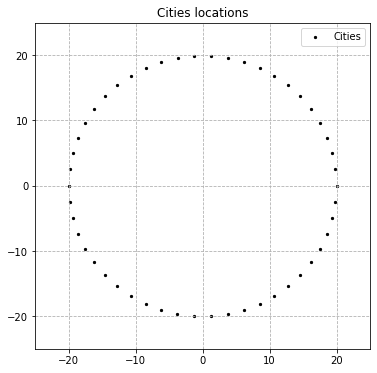
\includegraphics[width = 6cm]{dots1_1.png} &
            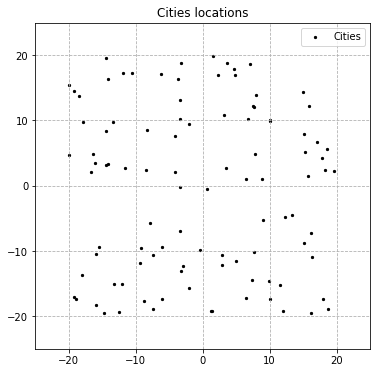
\includegraphics[width = 6cm]{dots2_1.png} \\
        \end{tabular}
        \label{image21}
        \caption{Примеры расположения городов на плоскости.}
    \end{figure}
    
    Города будем изображать точками на плоскости. Для проверки алгоритмов 
    будем использовать две карты (рис.~\ref{image21}.1). На левой 50 городов 
    расположены по кругу, на правой 100 городов разбросаны по плоскости 
    случайно. Пример слева является тривиальным, оптимальный маршрут обхода 
    всех точек (по кругу) очевиден.
    
    \begin{figure}[h!]
        \center
        \begin{tabular}{cc}
            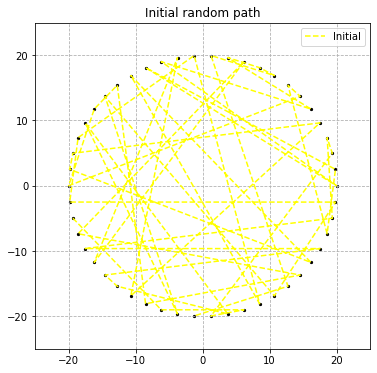
\includegraphics[width = 6cm]{dots1_2.png} &
            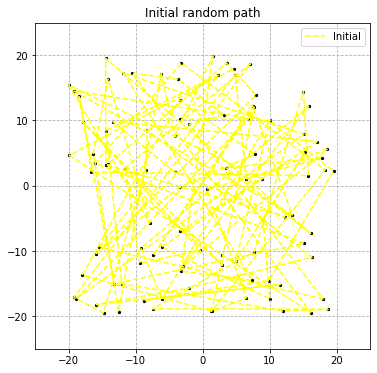
\includegraphics[width = 6cm]{dots2_2.png} \\
        \end{tabular}
        \label{image22}
        \caption{Инициализация случайными маршрутами.}
    \end{figure}
    
    Изначально пути между городами проложены случайным образом 
    (рис.~\ref{image22}.2). Такие конфигурации не являются оптимальными 
    (длина маршрута для первой: 1230 , для второй: 2220), и поэтому мы будем 
    оптимизировать их методом имитации отжига и алгоритмом муравьиной 
    колонии.
    
    \section{Алгоритм муравьиной колонии}
    
    \textbf{Муравьиный алгоритм}~(алгоритм оптимизации подражанием 
    муравьиной колонии, англ. \textit{ant colony optimization}, ACO)~--~один 
    из эффективных полиномиальных алгоритмов для нахождения приближённых 
    решений задачи коммивояжёра, а также решения аналогичных задач поиска 
    маршрутов на графах. Суть подхода заключается в анализе и использовании 
    модели поведения муравьёв, ищущих пути от колонии к источнику питания, и 
    представляет собой метаэвристическую оптимизацию.
    
    В основе алгоритма лежит поведение муравьиной колонии~--~маркировка 
    более удачных путей большим количеством феромона. Работа начинается с 
    размещения муравьёв в вершинах графа (городах), затем начинается 
    движение муравьёв~--~направление определяется вероятностным методом, на 
    основании формулы (\ref{eq31}).
    
    \begin{equation}
        P_{i} = \frac{l_{i}^{q} \cdot f_{i}^{p}}{\sum_{k=0}^{N} l_{k}^{q} 
            \cdot f_{k}^{p}}
        \label{eq31}
    \end{equation}
    
    В дальнейшем нам пригодятся величины $p$ и $q$. Они характеризуют 
    <<жадность>> и <<стадность>> алгоритма. Одним из важных параметров 
    является количество муравьев $K$ (количество запусков итераций 
    алгоритма), а так же <<скорость испарения ферамона>>.
    
    Проверим работоспособность алгоритма на тривиальном примере 
    (рис.~\ref{image21}.1 слева). Количество итераций $K = 200$, $p = 1$, $q 
    = 2$. Результат работы представлен на рис.~\ref{image33}.3 слева.
    
    \begin{figure}[h!]
        \center
        \begin{tabular}{cc}
            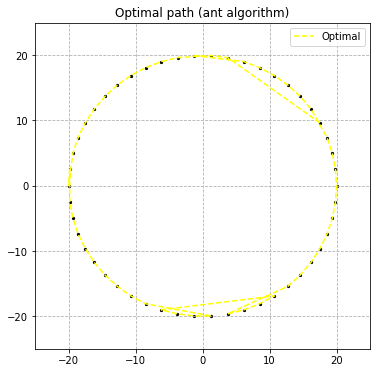
\includegraphics[width = 6cm]{dots1_2_1.png} &
            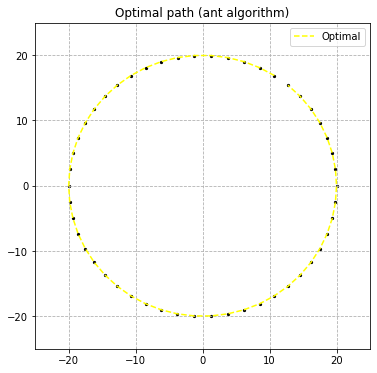
\includegraphics[width = 6cm]{dots1_2_2.png} \\
        \end{tabular}
        \label{image33}
        \caption{Оптимизация муравьиным алгоритмом для $q = 2$ слева и $q = 
            5$ справа.}
    \end{figure}
    
    Видно, что решение не является оптимальным. Теперь увеличим значение $q$ 
    до 5 (рис.~\ref{image33}.3 справа). Получили искомое решение тривиальной 
    задачи Коммивояжера. Алгоритм работает корректно.
    
    Теперь рассмотрим более сложный пример (рис.~\ref{image21}.1 справа). 
    Запустим алгоритм с теми же параметрами (рис.~\ref{image34}.4 слева). 
    Длина маршрута составит 399.9.
    
    Теперь будем считать, что $q = 7, K = 500$ (рис.~\ref{image34}.4 
    справа). Получим уже другой маршрут, но он ближе к оптимальному, т.к. 
    его длина равна 365.3.
    
    \begin{figure}[h!]
        \center
        \begin{tabular}{cc}
            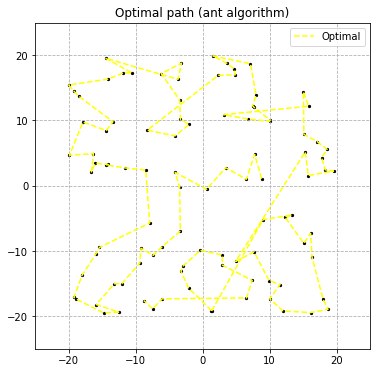
\includegraphics[width = 6cm]{dots2_2_1.png} &
            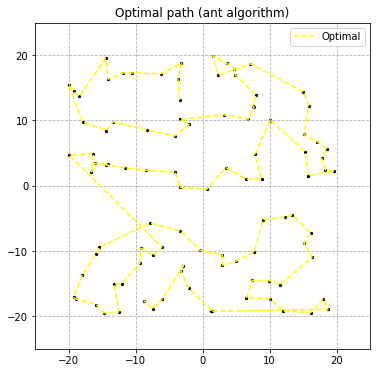
\includegraphics[width = 6cm]{dots2_2_2.png} \\
        \end{tabular}
        \label{image34}
        \caption{Оптимизация муравьиным алгоритмом для $q = 5, K = 200$ 
            слева и $q = 7, K = 500$ справа.}
    \end{figure}
    
    То есть есть смысл менять начальные параметры алгоритма, это позволяет улучшить результат.
    
    \section{Метод имитации отжига}
    
    Алгоритм имитации отжига (англ. \textit{Simulated annealing})~--~общий 
    алгоритмический метод решения задачи глобальной оптимизации, особенно 
    дискретной и комбинаторной оптимизации. Алгоритм основывается на 
    имитации физического процесса, который происходит при кристаллизации 
    вещества, в том числе при отжиге металлов.
    
    Проверим работоспособность алгоритма на тривиальном примере 
    (рис.~\ref{image21}.1 слева). Считаем $t_{0} = 100, t_{1} = 1, alpha = 
    0.95$. Результат работы представлен на рис.~\ref{image45}.5 слева.
    
    \begin{figure}[h!]
        \center
        \begin{tabular}{cc}
            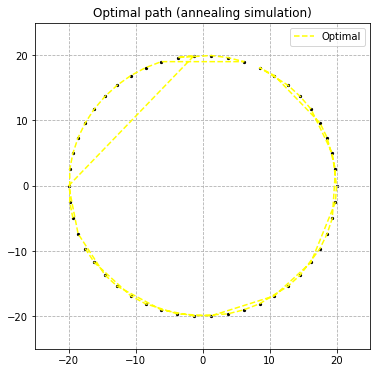
\includegraphics[width = 6cm]{dots1_2_3.png} &
            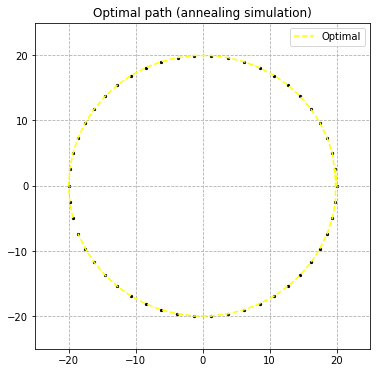
\includegraphics[width = 6cm]{dots1_2_4.png} \\
        \end{tabular}
        \label{image45}
        \caption{Оптимизация методом имитации отжига для $alpha = 0.95$ 
            слева и $alpha = 0.98$ справа.}
    \end{figure}
    
    Видно, что решение не является оптимальным. Теперь увеличим значение 
    $alpha$ до 0.98 (рис.~\ref{image45}.5 справа). Получили искомое решение 
    тривиальной задачи Коммивояжера. Алгоритм работает корректно.
    
    Теперь рассмотрим второй пример (рис.~\ref{image21}.1 справа). 
    Запустим алгоритм с теми же параметрами (рис.~\ref{image46}.6 слева). 
    Длина маршрута составит 489.
    
    Далее будем считать, что $alpha = 0.99, t_{0} = 150$ (рис.~\ref{image46}.6 справа). Получим уже другой маршрут, но он ближе к оптимальному, т.к. его длина равна 395.3.
    
    \begin{figure}[h!]
        \center
        \begin{tabular}{cc}
            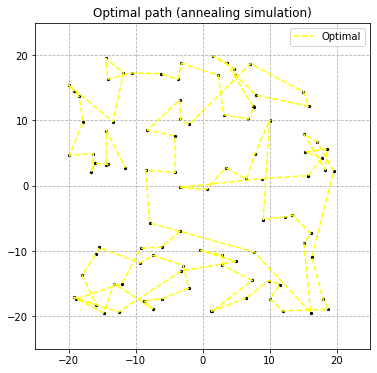
\includegraphics[width = 6cm]{dots2_2_3.png} &
            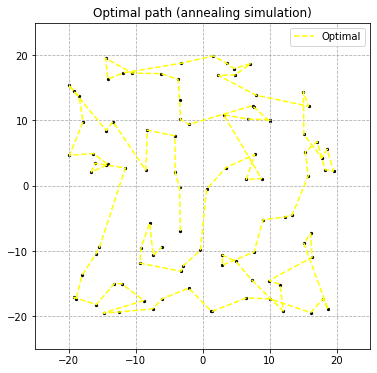
\includegraphics[width = 6cm]{dots2_2_4.png} \\
        \end{tabular}
        \label{image46}
        \caption{Оптимизация методом имитации отжига для $alpha = 0.98, 
            t_{0} = 100$ слева и $alpha = 0.99, t_{0} = 150$ справа.}
    \end{figure}
    
    То есть есть смысл менять начальные параметры алгоритма, это позволяет улучшить результат.
    
    \section{Сравнение алгоритмов}
    
    Нетрудно заметить, что во всех случаях маршрут, который строит 
    муравьиный алгоритм оказывается оптимальней того, который получается в 
    методе имитации отжига. Более того последний справляется с задачей 
    намного медленнее первого. Поэтому можно сказать, что для решения задачи 
    Коммивояжера лучше подходит алгоритм муравьиной колонии (хотя у каждого метода есть свои преимущества и 
    недостатки). 
    
\end{document}